\chapter{Improving the Model}\label{chap:model_improvements}

In this chapter, I use the insights from Chapter~\ref{chap:crnn} to improve the \emph{CRNN} and address questions raised by the literature. I perform a series of experiments to test improvements to the model, evaluate a selection of models on the test set and perform qualitative analysis of the model's outputs.

Many of these experiments introduce new hyperparameters. I choose these hyperparameters in a greedy fashion and keep them as specified unless stated otherwise. While the assumption of independence between hyperparameters is certainly wrong, it is computationally infeasible to perform a full hyperparameter search.

I first conduct experiments verifying that CQTs are the best features for ACR and that a hop length of $4096$ is appropriate. These experiments are left to Appendix~\ref{sec:spectrogram-results} for brevity. To summarise, CQTs achieve $10\%$ greater accuracy than other spectrogram variants and any hop length less than $4096$ achieves similar results. Thus, I proceed with CQTs and a hop length of $4096$.

\section{Decoding}\label{sec:decoding}

As observed in~\ref{sec:smoothness}, the \emph{CRNN} predicts $168$ transitions per song as opposed to the $104$ seen in the ground truth data. I implement a decoding step over the frame-wise probability vectors to smooth predicted labels. Common choices for decoding models include a conditional random field (CRF)~\citep{ACRLargeVocab1, BTC} and a hidden Markov model (HMM)~\citep{BalanceRandomForestACR}. 

I first implement a HMM. The HMM treats the frame-wise probabilities as emission probabilities and the chord labels as hidden states. \citet{CQTvsChroma} note that using a transition matrix with homogeneous off-diagonal entries in the transition matrix performs similarly to using a learned transition matrix. I adopt such a transition matrix for this HMM, with a parameter $\beta$ denoting the probability of self-transition and all other transition probabilities equal to $\frac{1-\beta}{C-1}$. Decoding then follows the Viterbi algorithm~\citep{Viterbi} over the summed forward and backward pass.

A plot of the effect of $\beta$ on the model's performance and the number of transitions per song is shown in Figure~\ref{fig:hmm_beta_search}. From this plot we conclude that smoothing has little affect on the performance of the model while successfully reducing the number of transitions per song to that of the true labels. I choose $\beta = 0.15$ for the remainder of experiments as it results in $102$ transitions per song while maintaining high performance. 

\begin{figure}[ht]
    \centering
    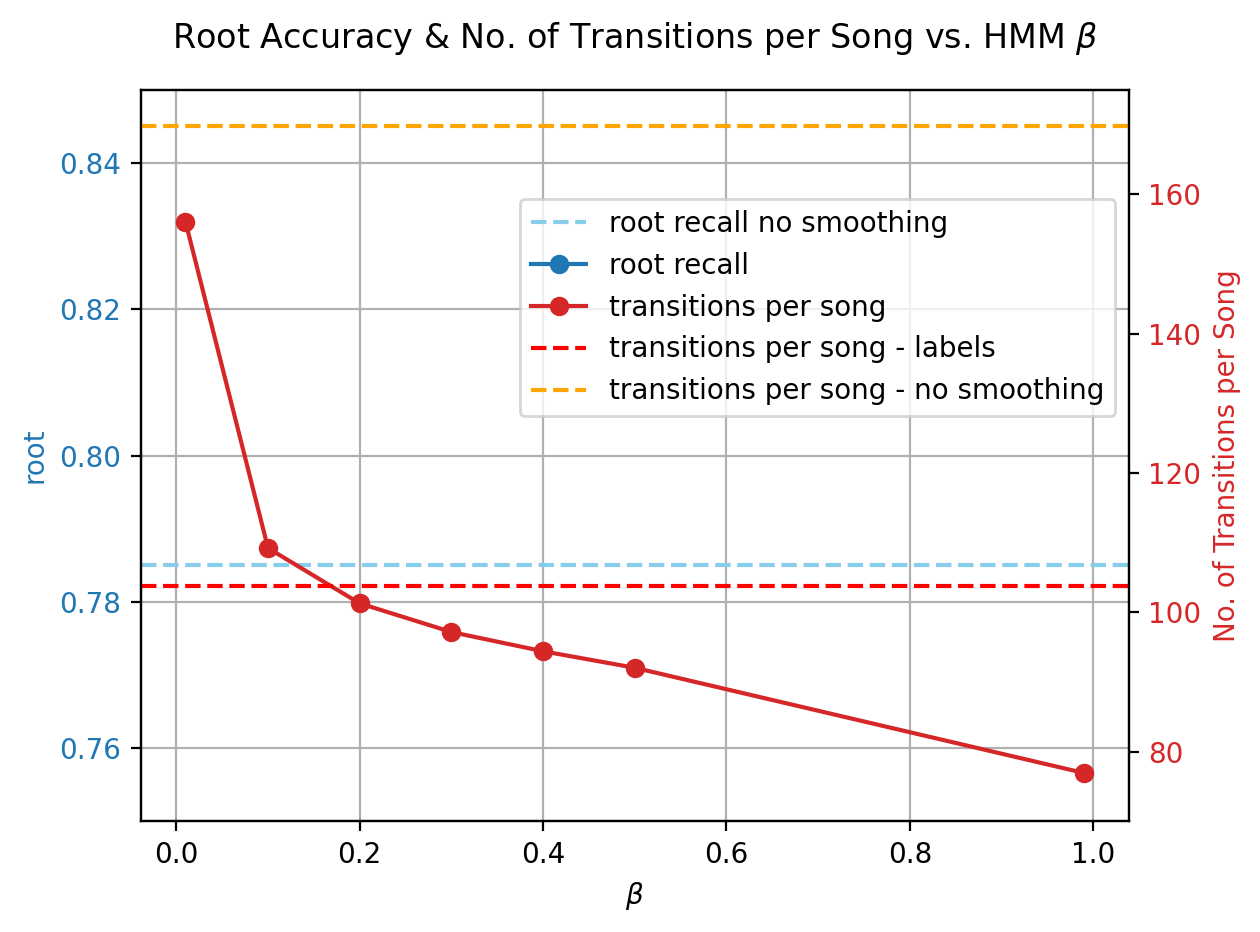
\includegraphics[width=0.8\textwidth]{figures/hmm_beta_vs_root_transitions.png}
    \caption{Effect of the HMM smoothing parameter $\beta$ on the \emph{CRNN} model. As we increase $\beta$, the number of transitions per song decreases. I choose $\beta = 0.15$ as it results in $102$ transitions per song, very close to the $104$ of the ground truth. Performance is stable across $\beta$ with a slight degradation for $\beta > 0.3$. Other performance metrics showed similarly stable results. }\label{fig:hmm_beta_search}
\end{figure}

The effect of the HMM on the incorrect regions previously discussed in Section~\ref{sec:smoothness} can be found in Appendix~\ref{app:histogram_over_region_lengths}. The HMM reduced the percentage of incorrect regions which are a single frame long from $26.7\%$ to $16.7\%$. A more intuitive way to see the effect of the HMM is to look at a section of a song which was the model previously predicted many chord transitions for. This is illustrated in Appendix~\ref{app:hmm_smoothing_effect}.

I also implement a linear chain CRF using \texttt{pytorch-crf}.\footnote{\url{https://github.com/kmkurn/pytorch-crf}} In contrast to the HMM, the CRF uses a learned transition matrix. Results comparing the HMM, CRF and no smoothing can be found in Table~\ref{tab:smoothers}. Both the CRF and HMM reduce the number of transitions per song to a similar level. The HMM outperforms the CRF, with $3.5\%$ greater accuracy. The HMM has almost identical performance to the model with no smoothing. I hypothesise that the learned transition matrix allows the model to overfit to the chord sequences in the training set. Regardless of the explanation, I proceed with HMM smoothing.

\begin{table}[ht]
    \centering
    \begin{tabular}{lcccccc}
        \toprule
        smoother & acc & root & third & seventh & mirex & transitions/song\\  
        \midrule
        none & \textbf{60.0} & \textbf{78.1} & \textbf{75.0} & \textbf{62.3} & \textbf{79.2} & 167 \\
        HMM & \textbf{60.0} &\textbf{78.1} & \textbf{75.0} & \textbf{62.3} & \textbf{79.2} & \textbf{102} \\
        CRF & 56.5 & 75.5 & 72.5 & 58.6 & 76.2 & 100 \\
        \bottomrule
    \end{tabular}
    \caption{Results for the HMM and CRF smoothing methods with the \emph{CRNN}. The HMM has almost identical performance to the model with no smoothing. However, it drastically reduces the number of transition per song to an acceptable level. The CRF performs notably worse than the HMM. }\label{tab:smoothers}
\end{table}

\section{The Loss Function}

\subsection{Weighted Loss}\label{sec:weighted_loss}

One of the biggest problems with the \emph{CRNN} is the low recall on rarer chord qualities. Two common methods for dealing with long-tailed distributions are weighting the loss function and over-sampling. \citet{CurriculumLearning} also explore the use of curriculum learning as form of re-sampling which we do not explore here because they report only minor performance gains. Sampling is explored by \citet{BalanceRandomForestACR} but they use a different model based on pre-computing chroma vectors and re-sampling these chroma vectors for use in training a random forest for frame-wise decoding. 

In our setting, re-sampling training patches of audio may be interesting to explore but is left as future work. It would require a complex sampling scheme as frames cannot be sampled independently. 

Weighting has been explored by \citet{ACRLargeVocab1}. We employ a similar but simpler implementation here. A standard method of weighting is to multiply the loss function by the inverse of frequency of each, with a parameter controlling the strength of the weighting. This is defined in Equation~\ref{eq:weighting}.

\begin{equation}\label{eq:weighting}
    w_c = \frac{1}{{(\text{count}(c) + 10)}^\alpha}
\end{equation}

Where $w_c$ is the weight for chord $c$, $\text{count}(i)$ is the number of frames with chord $c$ in the dataset and $\alpha$ is a hyperparameter controlling the strength of weighting. $\alpha=0$ results in no weighting and increasing $alpha$ increases the severity of weighting. I add $10$ in the denominator to avoid dividing by $0$ and to diminish the dominating effect of chords with very few occurrences. I then define normalised weights $w_c^*$ in Equation~\ref{eq:weighted_loss} so that the learning rate can remain the same.

\begin{equation}\label{eq:weighted_loss}
    w_c^* = \frac{w_c}{s} \text{ where } s = \frac{\sum_{c\in \mathcal{C}} \text{count}(c)\cdot w_c}{\sum_{c\in \mathcal{C}} \text{count}(c)}
\end{equation}

Where $\mathcal{C}$ is the set of all chords in the vocabulary. This keeps the expected weight over samples at $1$ such that the effective learning rate remains the same. These values are calculated over the training set. I test values of $\alpha$ in the set \{0, 0.05, 0.1, \ldots, 0.95, 1\}. The plot in Figure~\ref{fig:weighted_loss} illustrates the effect of the weighting on the model's performance. I find that increasing $\alpha$ improves \texttt{acc}\textsubscript{class} but decreases \texttt{root} accuracy. Choosing $\alpha = 0.3$ maximises \texttt{acc}\textsubscript{class} without hurting root accuracy which I carry forward to subsequent experiments.

\begin{figure}[H]
    \centering
    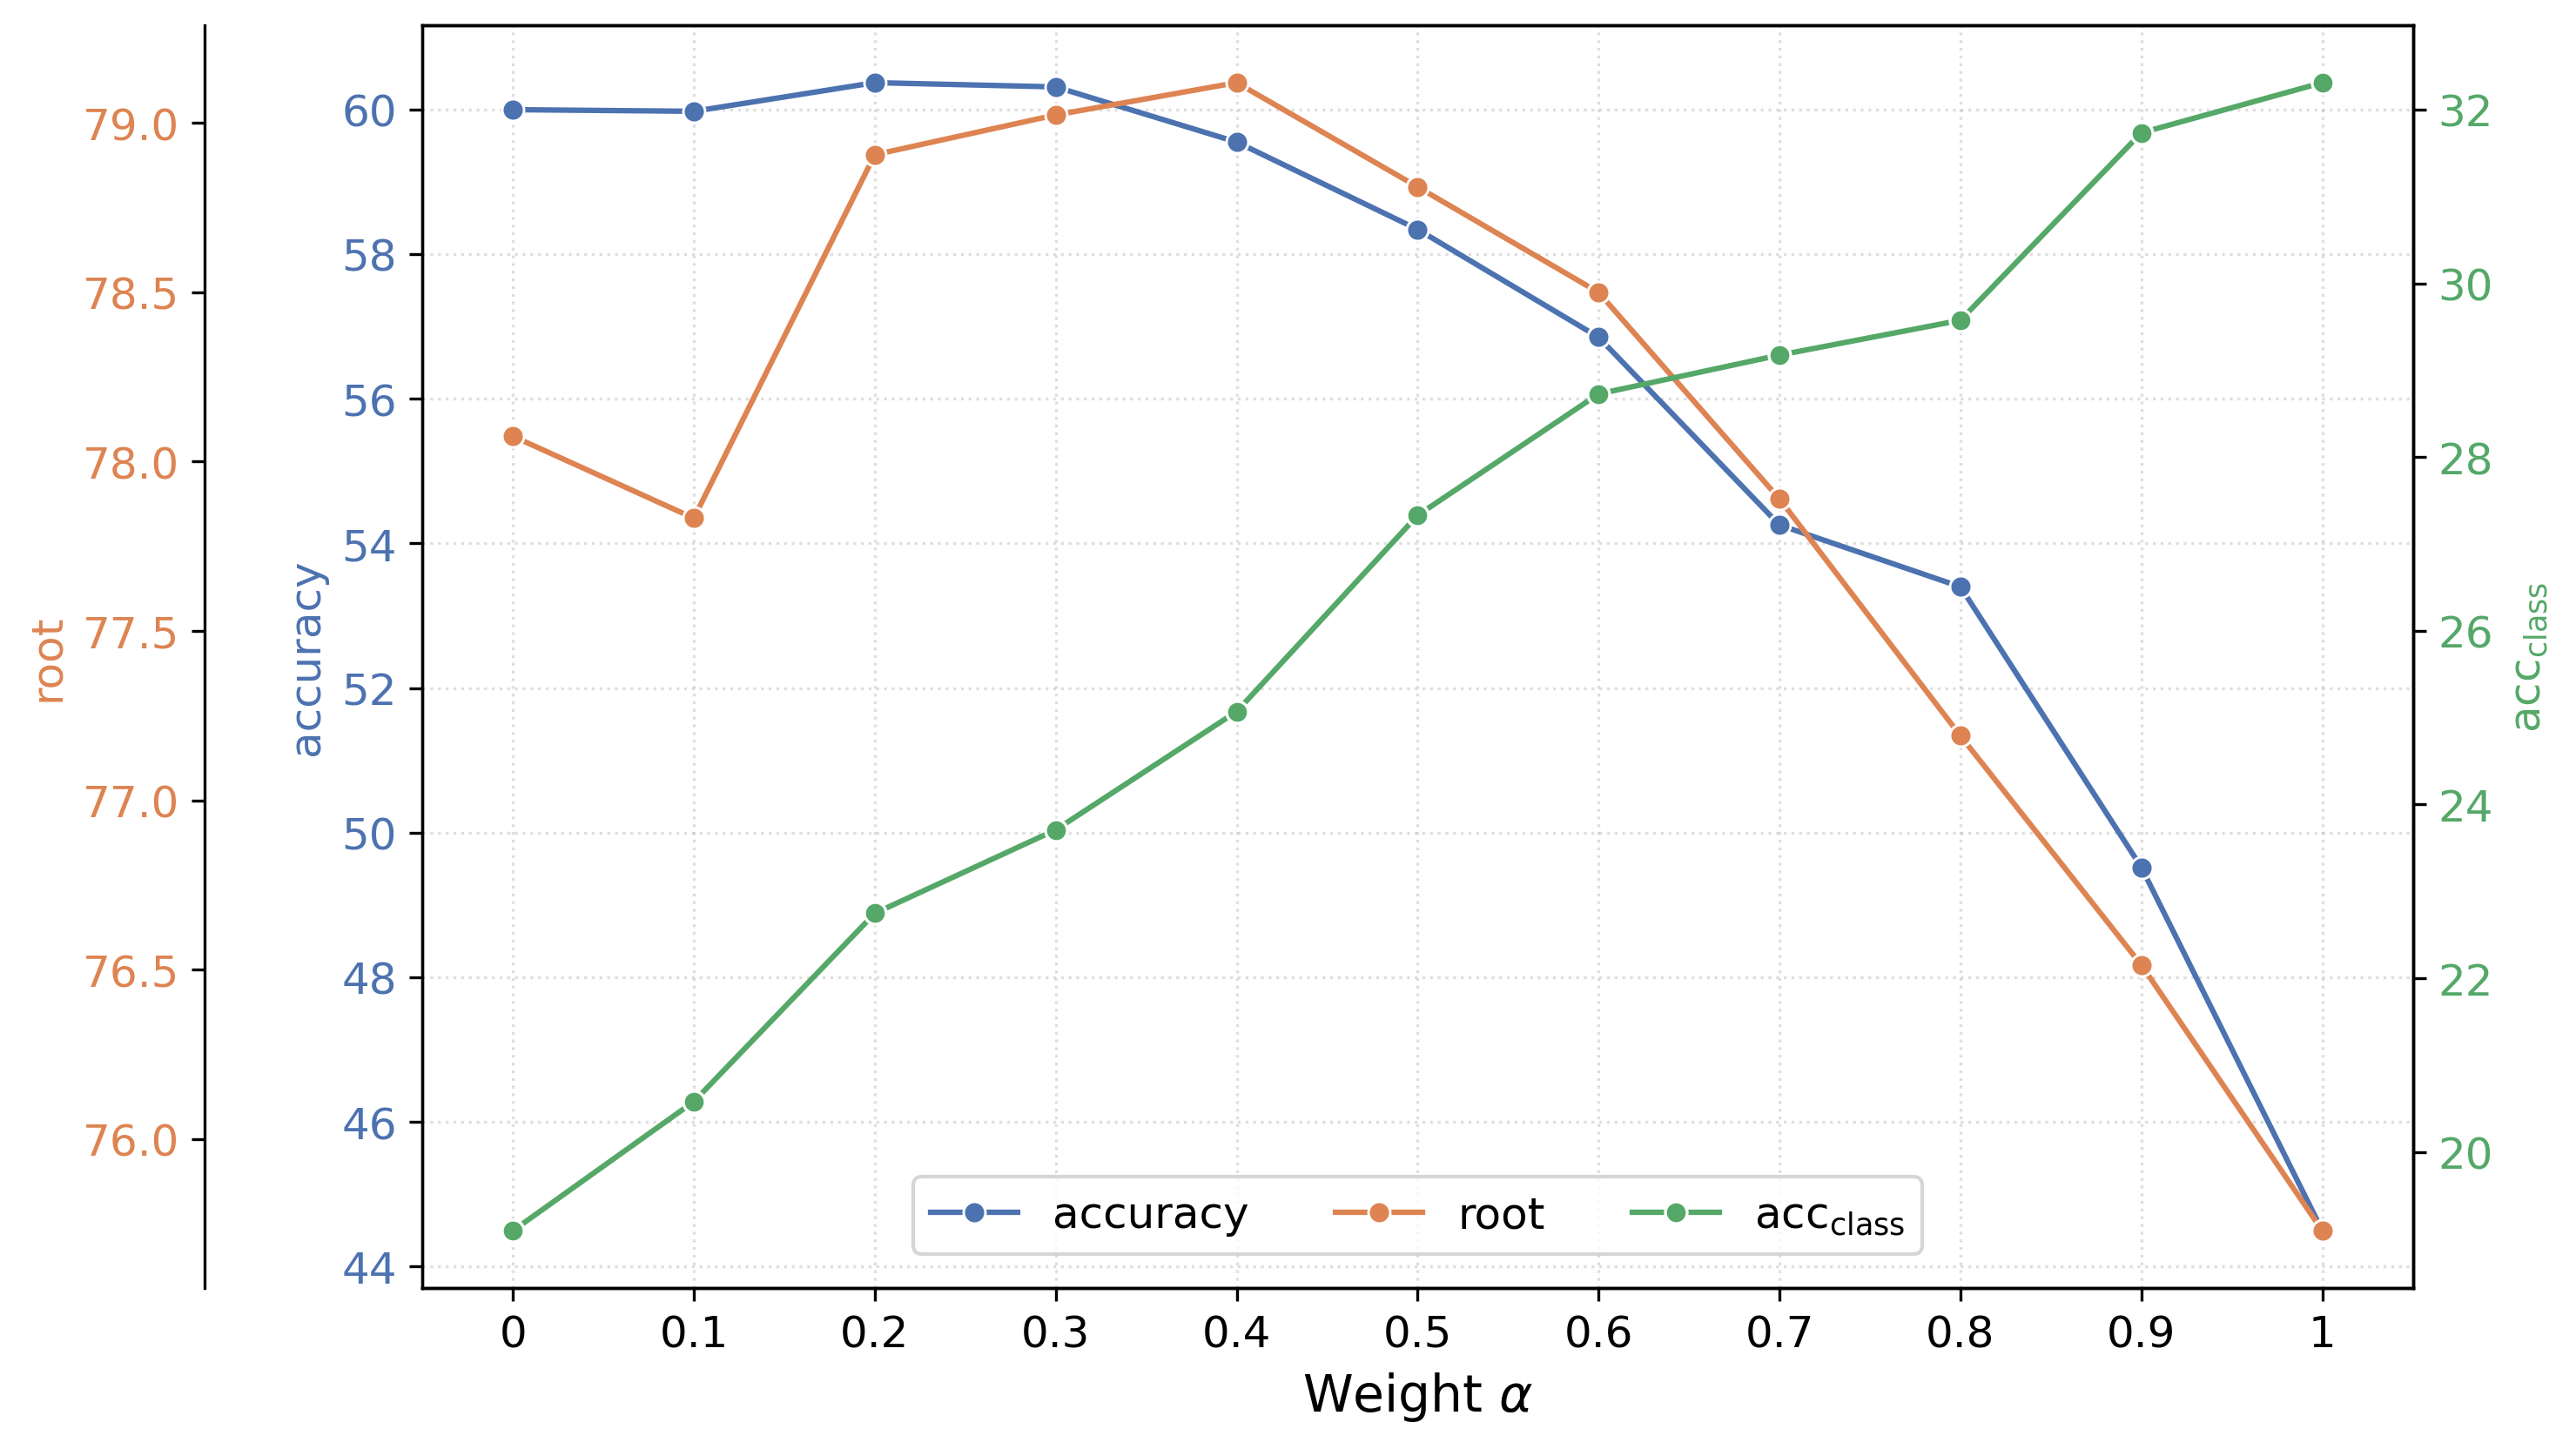
\includegraphics[width=0.8\textwidth]{figures/weight_alpha_search_trim.png}
    \caption{Effect of weighted loss on the \emph{CRNN} model with varying $\alpha$. As we increase $\alpha$, \texttt{acc}\textsubscript{class} improves accuracy and \texttt{root} decreases. I claim there is a sweet-spot where very little overall performance is sacrificed for better class-wise accuracies. I choose this to be $\alpha = 0.3$. The \texttt{root} and \texttt{third} metrics improve and less than $3\%$ is lost on other metrics while mean class-wise accuracy improves by $6\%$.}\label{fig:weighted_loss}
\end{figure}

For further insight, a plot of the differences between a confusion matrices with and without weighted loss can be found in Appendix~\ref{app:weighted_loss_confusion_matrix}. Notably, recall on most qualities increases, with recall on major7 doubling to $0.34$. The weighted model predicts $2.2$ times fewer \texttt{X} symbols which may explain how it increases recall on these rarer qualities without sacrificing on accuracy. 

Weighting the loss function also increased the number of transitions predicted per song slightly. This may be because occasional sharp gradient updates cause more extreme probability outputs. I increase the HMM smoothing parameter $\beta$ to $0.2$ to bring the number of transition per song to $104$.

\subsection{Structured Loss}\label{sec:structured_loss}

\citet{StructuredTraining} propose a structured loss function which they claim improves performance on the \emph{CRNN} model. They introduced additional targets of the root, bass and pitch classes. I follow a similar method but do not include the bass as the current chord vocabulary does not consider inversions. The idea behind this loss term is to explicitly task the model with identifying the components of a chord that we care about. This can allow the model to exploit structure in the chord vocabulary such as shared roots and pitch classes, rather than all symbols being predicted independently.

The root can be any of the 12 notes in the Western chromatic scale, \texttt{N} or \texttt{X}, creating a 14-dimensional classification problem. The 12 pitch classes each represent a single binary classification problem. Two fully connected layers calculate a 14-dimensional vector and 12-dimensional vector from the hidden representation outputted from the GRU for the root and pitch classes respectively. Finally, these representations are concatenated with the original output of the model and fed to the final fully connected layer to predict the chord symbol.

The mean cross-entropy loss is calculated in each case. These are then summed to from the \emph{structured loss}. Finally, a linear combination of the structured loss and the original loss is calculated. The final loss is a convex combination of the original loss and the structured loss as defined in Equation~\ref{eq:structured_loss}.

\begin{equation}\label{eq:structured_loss}
    L = \gamma L_{chord} + (1-\gamma)(L_{root} + L_{pitch})
\end{equation}

Where $L$ is the overall loss, $L_{chord}$ is the cross-entropy loss over chords symbols, $L_{root}$ is the cross-entropy loss targeting the root, $L_{pitch}$ is mean binary cross-entropy over each of the pitch classes. $\gamma$ is a hyperparameter controlling the weighting of the original loss. 

I test models with $\gamma\in\{0, 0.1 \ldots 0.9\}$. Choosing $\gamma=0.7$ improves accuracy by $1.3\%$ while \texttt{mirex} worsens by $0.3\%$. Accuracy with \texttt{third} increases by $1.7\%$ and on \texttt{seventh} by $1.3\%$. Generally, greater $\gamma$ improves accuracy metrics while \texttt{mirex} results are noisy. A plot of the trend can be found in Appendix~\ref{fig:structured_loss} but does not provide further insight. I keep $\gamma=0.7$ going forward based on peak accuracy. 

\section{Generative Features}\label{sec:generative_features}

\citet{MelodyTranscriptionViaGenerativePreTraining} use generative features extracted from Jukebox~\citep{Jukebox} to improve performance for melody transcription. They also produce a chord transcription model using the same methodology but do not report results. I decide to test generative features using MusicGen~\citep{MusicGen} as a feature extractor. This was for several reasons. MusicGen is a newer model. It has several different sizes of model which could be tested against each other as an experiment on the complexity of the model. It has a fine-tuned variant called MusiConGen~\citep{MusiConGen} which is used for synthetic data generation in Section~\ref{sec:synthetic_data}. All model weights are available on the HuggingFace Hub.\footnote{\url{https://huggingface.co/docs/hub/en/index}} Finally, its training data was properly licensed, unlike Jukebox. I leave the results of Jukebox for future work. Details of the feature extraction process are left to Appendix~\ref{app:generative_feature_extraction} for the interested reader.

As the representations are $2048$-dimensional, it is computationally infeasible to feed this directly into the GRU. Instead, I project these vectors down to a power of $2$, from $16$ to $1024$, using fully connected layers. The best representation is with $64$ dimensions although results show no clear trend. Results are left to Appendix~\ref{app:projection_dimensionality}.

I test different variants of MusicGen including musicgen-large (3.3B parameters), musicgen-small (330M), musicgen-melody (1.5B) and MusiConGen (1.5B). I also test different reductions of the four `codebooks' outputted by the language model including taking each codebook on its own, taking the element-wise mean across codebooks or the concatenation of all four. For further details on codebooks, see the work of \citet{MusicGen}. The best model was found to be musicgen-large and the best reduction to average over the four codebooks. However, results were all close and are left to Appendices \ref{app:generative_feature_extraction_models} and \ref{app:generative_feature_extraction_reductions} for lack of importance.

% It might be argued that it is better to use musicgen-small to save on computational cost but the dimensionality of the codebooks is the same across all model variants. Once the features have been extracted, they are all equally as expensive to train on.

It is surprising that the concatenated representation performs worse than the averaged representation as it contains at least as much information. However, if the information provided by each of the codebooks is largely the same then there are no reasons that the concatenated representation should perform better and training with Adam may simply find a worse minima. Training on $8192$-dimensional vectors is also computationally expensive.

To test whether or not these features help when compared with a CQT, I test with the CQT only, generative features only and a concatenation of the two. The results are shown in Table~\ref{tab:gen_feature_comparison}. Although the generative features perform worse than the CQT, they clearly contain information useful for chord recognition with an accuracy of $58.7\%$. When the CQT and generative features are used together, performance remains largely the same. This experiment was run multiple times, with similar results each time. There is no clear evidence that the generative features provide any benefit over just using the CQT. 

This is surprising as \citet{MelodyTranscriptionViaGenerativePreTraining} claim that generative features are better than hand-crafted features for the related task of melody recognition. However, they only compare to mel-spectrograms which may perform as well as CQTs for melody recognition. Observations here cast doubt on the validity of their claims. It may be the case that features extracted from other generative models such as Jukebox~\citep{Jukebox} or MusicLM~\citep{MusicLM} perform better. The comparison is left for future work.

Given the lack of improvement and the drastically increased computational cost associated with extracting features and training the model, I do not proceed with using generative features.

\begin{table}
    \centering
    \begin{tabular}{lccccc}
        \toprule
        features & accuracy & root  & third & seventh & mirex \\  
        \midrule
        gen$\cdot$CQT  & \textbf{61.0}     & \textbf{80.3}  & \textbf{77.0}  & \textbf{63.3}    & 78.4  \\
        gen      & 58.7     & 77.6  & 74.3  & 60.9    & 77.5  \\
        CQT      & \textbf{61.0}     & 79.8  & 76.8  & 63.2    & \textbf{79.3}  \\
        \bottomrule
    \end{tabular}
    \caption{Comparison of CQT and generative features with a concatenation of the two, denoted as gen$\cdot$CQT. The concatenation performs the best on most metrics, but not by enough to claim that it is meaningfully better. }\label{tab:gen_feature_comparison}
\end{table}

\section{Pitch Augmentation}\label{sec:pitch-augmentation}

Pitch augmentation has been done in other works on chord recognition, either on the CQT~\citep{ACRLargeVocab1} or on the audio~\citep{BTC,StructuredTraining}. Although similar, these are not identical transformations. Shifting the CQT takes place after discarding phase information and leaves empty bins behind whereas audio pitch shifting can introduce other artefacts intended to preserve harmonic structure and maintain phase information. I implement both methods and compare.

When a sample is drawn from the training set, it is shifted with probability $p$. The shift is measured in semitones in the set $\{-5,-4\ldots -1, 1, \ldots 6\}$ with equal probability of each shift. This means there is 12 times as much training data. Convergence was still reached in 150\,epochs. Shifting the CQT matrix is done by moving all items up or down by the numbers of bins corresponding to the number of semitones in the shift. The bins left behind filled with a value of -80dB. Audio shifting is done with \texttt{pyrubberband}.\footnote{\url{https://github.com/bmcfee/pyrubberband}}. CQTs are then calculated on the shifted audio. A plot of the effect of the shift probability $p$ on the model's performance can be found in Figure~\ref{fig:pitch_augmentation}.

Results show a clear trend that increasing $p$ improves performance. Shifting the audio provides a very similar effect to simply shifting the CQT. Choosing $p=0.9$ results in a $2.1\%$ increase in accuracy. The \texttt{mirex} score breaks the trend with performance varying over different values for $p$. \texttt{acc}\textsubscript{class} also improves by over $2\%$. This can be explained by the model becoming becoming root-invariant. With $p=0.9$, all potential roots become close to equally likely. I proceed with pitching shifting with $p=0.9$ on the CQT for the remainder of the experiments as it is computationally cheaper than shifting the audio.

\citet{StructuredTraining} claim an increase of $5\%$ on the median across most metrics. I do not find such a large effect here. Nonetheless, it is clear that pitch shifting is a useful augmentation.

Note that the weights for the weighted loss are calculated based on \emph{expected} counts, taking the shift probability $p$ into account. I also test shifting on both the CQT and audio but results are not any different than either method alone. Unfortunately, it was not computationally feasible to test pitch shifting with generative features as the feature extraction over $12 * 1210 = 14,520$ songs is too expensive.

\begin{figure}[H]
    \centering
    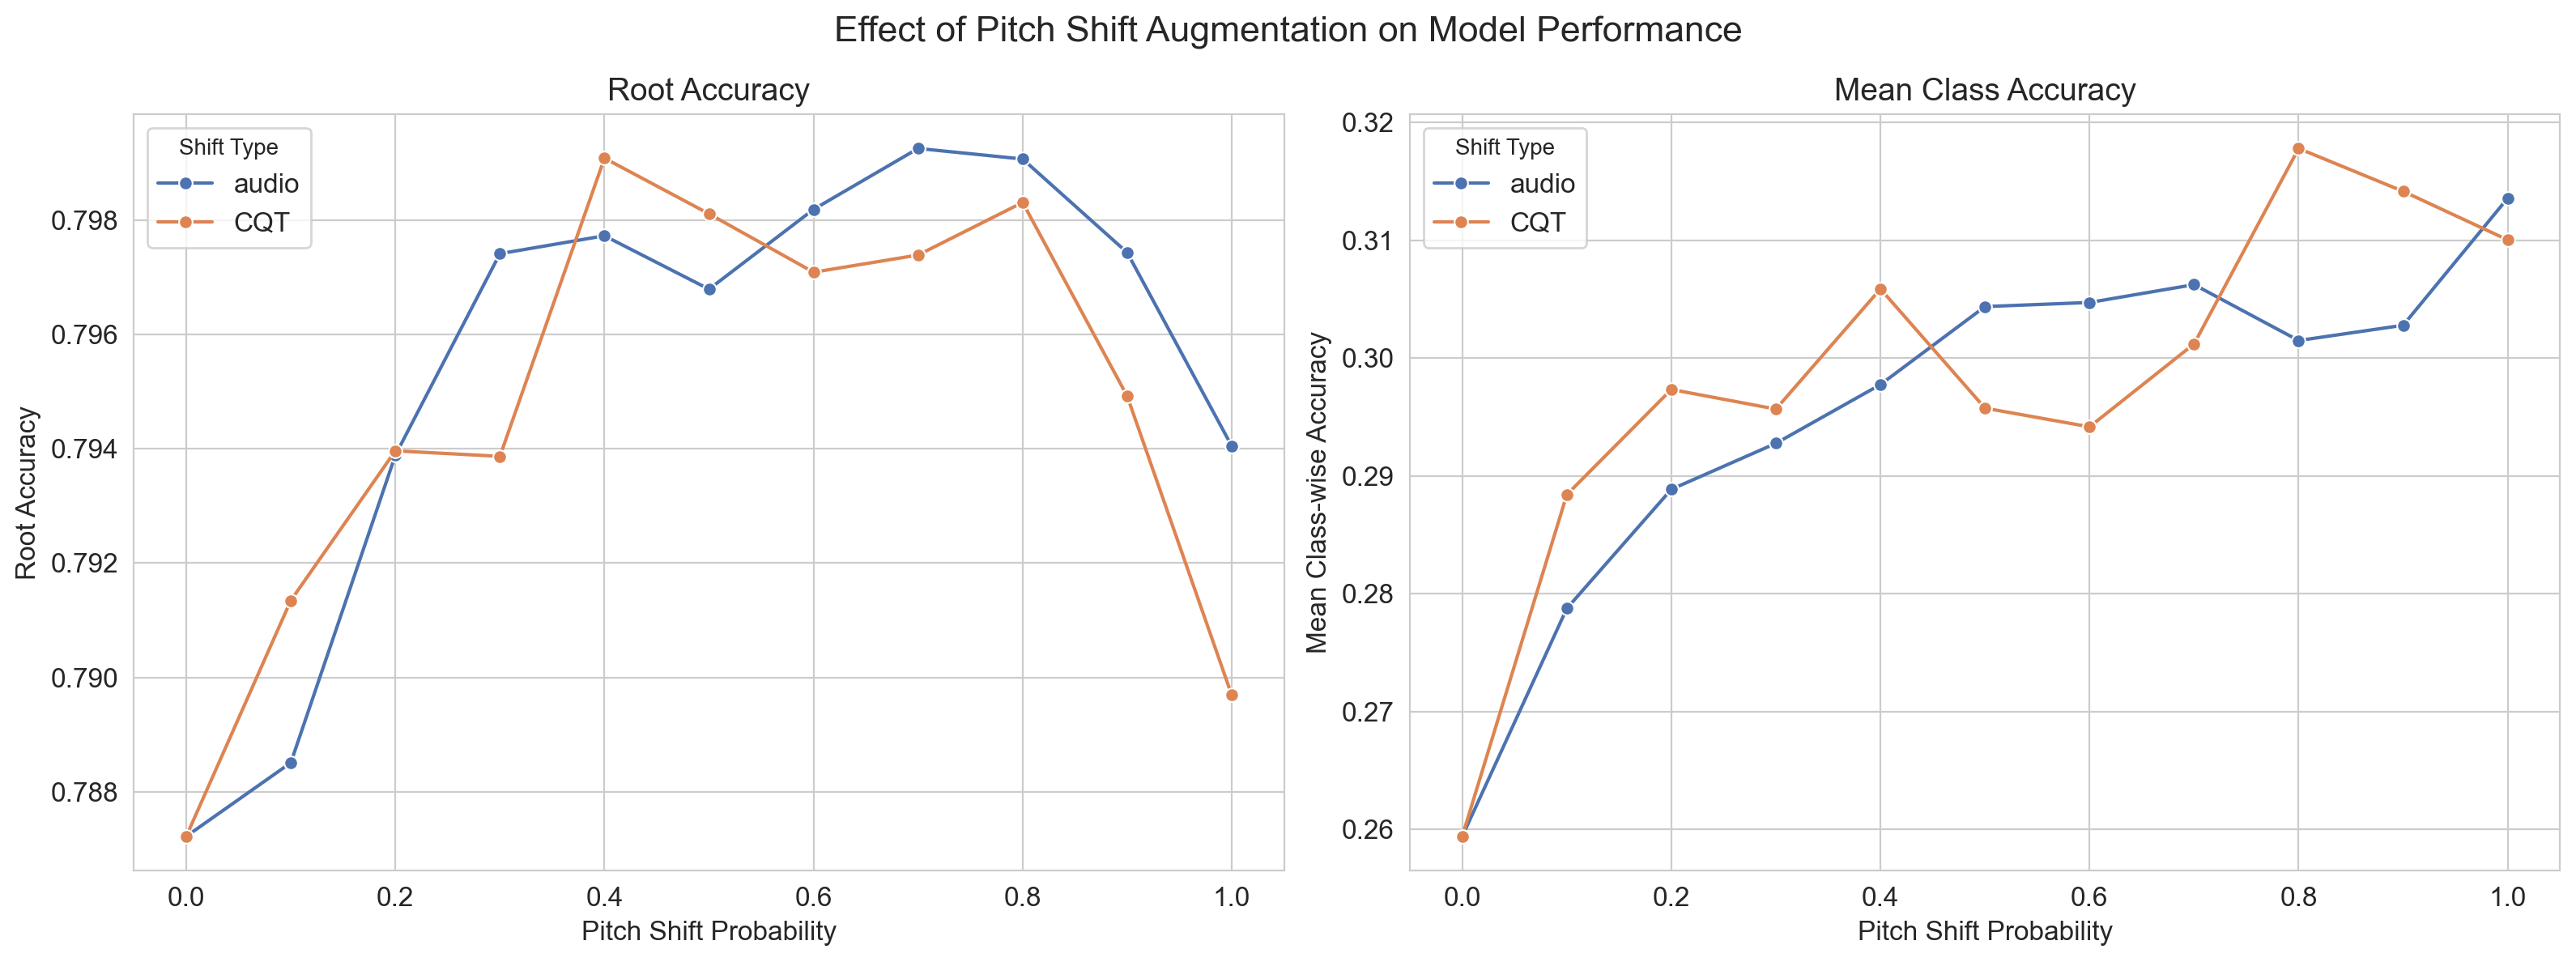
\includegraphics[width=1.0\textwidth]{figures/pitch_shift_analysis.png}
    \caption{Effect of pitch shift probability $p$ on \texttt{root} (left) and acc\textsubscript{class} (right). Pitch shifting provides a clear increase in performance. Shifting the audio or the CQT has a similar effect. I choose $p=0.9$ which is close to making the model root-invariant.}\label{fig:pitch_augmentation}
\end{figure}


\section{Synthetic Data Generation}\label{sec:synthetic_data}

Given the success of pitch augmentation for ACR, it is sensible to look for other sources of data. Further augmentation is possible such as adding noise and time-stretching. However, these do not provide new harmonic structure or create new instances of rare chords so I do not explore these here. Instead, I look to generate new data.  Generation would be possible through automatic arrangement, production and synthesis. However, this is a complex task, requires a lot of human input and is unlikely to produce sufficient variety of timbres, instrumentation arrangement. Instead, I use a recent chord-conditioned generative model called MusiConGen~\citep{MusiConGen}. I use this over CocoMulla~\citep{CocoMulla} as the method of chord-conditioning has a simpler interface, doesn't require reference audio and the authors claim that it adheres more closely to its conditions. Indeed they feed the outputted audio through BTC~\citep{BTC} and find a \texttt{triads} score of $71\%$ using the chord conditions as the ground truth. While far from perfect, it suggests the model is able to generate audio that mostly lines up with the chord conditions.

I generate $1210$ songs, each $30$ seconds long, to mimic the size of the \emph{pop} dataset. I refer to this dataset as \emph{synth}. This is split into a train, validation and test split in the same fashion as for the \emph{pop} dataset. To generate a larger order of magnitude of songs would require a lot of compute. While the model does support auto-regressive generation for longer audio, I find that its outputs become incoherent using the provided generation functions. It also sometimes produces incoherent output with $30$ seconds but this was much less common.

To generate a song, I sample a BPM from a normal distribution with mean $117$ and standard deviation $27$, clipped to lie in the range $[60,220]$. These values were calculated from the training set. I then sample a song description from a set of $20$ generated by ChatGPT. The descriptions outline a genre, mood and instrumentation. Descriptions include only jazz, funk, pop and rock which were all part of the fine-tuning training set for MusiConGen. Note that the model does not output melodic vocals, owing to the lack of vocal music in the pre-training and fine-tuning data. Finally, I generate a jazz chord progression using the theory of functional harmony~\citet{GenerativeGrammarJazz}. Details of this process can be found in Appendix~\ref{app:jazz_chord_progression_generation}. The process generates a very different chord distribution than the one in \emph{pop} with many more instances of upper extensions and rare qualities. This is intended to provide the model with many more instances of rare chords. 

To offset this distribution shift, I calibrate the probabilities outputted by the model. To encourage root-invariance, calibration terms are averaged over roots for each quality. The details of calibration are described in Appendix~\ref{app:calibration} with a figure showing the calibration terms for each quality. This figure shows that the rarer qualities are much more common in the synthetic data.

Outputs from MusiConGen were manually inspected. In general, the outputs are good. They consistently stick to the provided BPM and usually stick to the chord conditions. Outputs are occasionally musically strange with jarring drum transients and unrealistic chord transitions. They also did not have an enormous variety in terms of timbre and instrumentation. Nonetheless, the majority of examples have sensible annotations that one would expect a human to be able to annotate well. 

I compare a model trained on only \emph{pop}, trained on only synthetic data and trained on both. While the latter results in more training data per epoch, convergence is always reached so these are fair comparisons. I test the models on both the \emph{pop} and synthetic data validation splits. Given the increased instances of rare chords in the synthetic data, I remove the weighting on the loss function for the models trained on synthetic data.

The results are shown in Table~\ref{tab:synthetic_data}. The model trained on both datasets performs very similarly to the model only trained on \emph{pop}. That is, the model has not overfitted to the synthetic data. However, it has also not improved performance. Training on any synthetic data drastically improves the accuracy on the \emph{synth} validation split. This is likely due to the unique chord distribution of the generated jazz progressions and the consistent instrumentation. The model trained on both datasets performs the best, with an accuracy of $51.0\%$.

\begin{table}[h]
    \centering
    \begin{tabular}{lcccc}
        \toprule
        training set & \emph{pop} acc & \emph{pop} third & \emph{pop} seventh & \emph{synth} acc \\  
        \midrule
        \emph{pop} & \textbf{62.1} & 77.7 & 64.4 & 24.2 \\
        \emph{synth} & 48.6 & 64.4 & 50.6 & 44.8 \\
        both & \textbf{62.1} & \textbf{77.9}  & \textbf{64.6} & \textbf{51.0} \\
        \bottomrule
    \end{tabular}
    \caption{Results for models trained on \emph{pop}, \emph{synth} and both together. Unsurprisingly models trained on \emph{pop} perform better on \emph{pop} and models trained on \emph{synth} perform better on \emph{synth}. The model trained on both does not to meaningfully better on the \emph{pop} validation split, but performance is increased on the \emph{synth} validation split. Training only on \emph{pop} results in an accuracy of just $24.2\%$ on \emph{synth}, much lower than reported by \citet{MusiConGen}. However, this may be due to the unrealistic distribution of chords in the generated sequences. }\label{tab:synthetic_data}
\end{table}

For further insight, the difference in confusion matrix over qualities is plotted in Appendix~\ref{app:cm_synthetic_data}. There are few clear trends. Recall on some rare qualities increases and decreases for others. Notably, recall on \texttt{min7} improves by $13\%$ and the model is much better at predicting the third in dominant and minor 7 chords. This is perhaps why the third and seventh accuracies increase slightly on the \emph{pop} validation set. 

While performance does not meaningfully improve on \emph{pop}, the lack of overfitting and the gain on the synthetic data provides hope that with further work and improved generative models, synthetic data could prove a useful tool for ACR. Given the lack of performance increase, I do not continue to train on synthetic data.

\section{Beat Synchronisation}\label{sec:beat-synchronisation}

Chords exist in time. Musicians interpret chords in songs as lasting for a certain number of beats, not a fixed length of time. In its current form, the model outputs frame-wise predictions. While these could be stitched together to produce a predicted chord progression or beat-wise predictions could be made as a post-processing step, I decide to implement a model that outputs beat-wise predictions directly. This allows the model to use information from the entire duration of the beat to make its prediction.

Following the methodology of \citet{MelodyTranscriptionViaGenerativePreTraining}, I first detect beats using \texttt{madmom}~\citep{madmom}. This returns a list of time steps where beats have been detected. I first verify that these beats are plausible. I perform a cross-correlation analysis with the chord transitions in a similar manner to Section~\ref{sec:data-integrity}. A histogram of maximum lags within a window of $0.3$ seconds can be found in Appendix~\ref{app:maximum_lag_cross_correlation_beats}. I find that almost all maximum lags occur within a window of $0.1$ seconds. To provide further evidence, I compute the maximum accuracy a model could attain if predicting chords at the beat level. This is done by iterating over each beat interval and assigning the chord with maximum overlap with the ground truth. This yields an accuracy of $97.1\%$. With these observations combined, I am satisfied that the estimated beats are accurate enough to be used.

To calculate features for a beat interval, I average all CQT features whose centre is contained within the interval. The CQT is calculated using a hop length of $1024$. The shorter hop length is used to minimise the effect of CQT frames with partial overlap with two beat intervals and ensures that each beat has many CQT frames associated with it. These representations have the added benefit of decreased computational cost as beats have a lower frequency than frames.

% \citet{MelodyTranscriptionViaGenerativePreTraining} task the model with producing predictions for every 1/16th of a beat. However, such fast transitions are not necessary for chord recognition. The possible accuracy of $97.1\%$ over beats suggests that the model need only predict once every beat interval.

I test the model with different divisions and groupings of beats. This is to test the assumption that the whole beats are fine-grained enough for the model to make good predictions. I include tests where beat intervals are sub-divided in two, in four, or beat intervals are joined into groups of two. I refer to this as the \emph{beat division}. I also test a \emph{perfect} beat division where the true chord transitions are taken as the beats. This is not a fair comparison as the model should not have access to true transition timings. However, it does provide an idea of how the model would fare if it could perfectly predict chord transitions. Note that HMM smoothing is removed for beat-wise models as it is no longer necessary.

Results are shown in Table~\ref{tab:beat_division}. Using beat-wise predictions does not affect performance compared to frame-wise predictions. The model also performs just as well with a beat division of $1$ as with a beat division of $1/2$ or $1/4$. The model performs worse with a beat division of $2$ though only loses $6\%$ accuracy. This suggests that most chord transitions occur at frequencies smaller than the beats produced by \texttt{madmom} but that sometimes the two are misaligned.

The model with `perfect' beat intervals performs slightly worse on accuracy metrics but attains a very high \texttt{mirex} score of $90.4\%$ which is the highest of any seen in the literature. This is a very promising result. Data from the CQT producing a \texttt{mirex} score of $90.4\%$ suggests provides hope for significant improvements in the field. Why the model performs worse on accuracy metrics is not clear. It may be because averaged features from longer time periods provide better information as to the pitch classes present but dampens signal regarding the root note. Indeed, the mean chord duration is $1.68$ seconds while a CQT frame is $0.093$ seconds. Why this effect is not observed when predicting at the beat-level is also not clear. Further analysis may lead to significant improvements on ACR.

\begin{table}[H]
    \centering
    \begin{tabular}{lccccc}
        \toprule
        beat division & acc & root & third & seventh & mirex \\  
        \midrule
        1/4                 & 62.3           & 81.3          & 78.3          & 64.5           & 79.6         \\
        1/2                 & \textbf{62.8}  & 81.5          & \textbf{78.6} & \textbf{65.1}  & 79.9         \\
        1                   & 62.3           & 81.3          & 78.1          & 64.6           & 80.0         \\
        2                   & 56.4           & 74.7          & 71.6          & 58.5           & 73.4         \\
        % 4 & 50.8           & 68.0          & 64.5          & 52.8           & 67.2         \\
        none                & 62.5           & \textbf{81.7} & 78.2          & 64.7           & 80.2         \\
        perfect             & 61.1           & 79.6          & 76.1          & 63.4           & \textbf{90.4}\\
        \bottomrule
    \end{tabular}
    \caption{Results for different beat divisions. The beat division of `none' refers to a frame-wise \emph{CRNN} with a hop length of $4096$ and HMM smoothing applied and `perfect' refers to intervals that are calculated from the labels. Note that this `perfect' model is not a fair test. Beat-wise predictions with beat intervals of $1$ and below see no decrease in performance compared to frame-wise predictions. Beat intervals greater than $1$ increasingly suffer from being forced to assign predictions to larger periods of time that may not line up with true chord transitions. Interestingly, a beat interval of 2 still performs relatively well. A notable result is the \texttt{mirex} score of the `perfect' model. A score of $90.4\%$ is the highest of any in the literature. Despite this, its accuracy does not improve. }\label{tab:beat_division}
\end{table}


\section{Final Results}\label{sec:test-set}

For final results, I retrain select models on the combined training and validation splits and test on the held out test split. This is an 80/20\% train/test split. I consider the original \emph{CRNN} with no improvements, the \emph{CRNN} with a weighted and structured loss and HMM smoothing, concatenating generative features with CQTs, pitch augmentation, beat-wise predictions, `perfect' beat-wise predictions and training on synthetic data. 

Results are shown in Table~\ref{tab:test_set}. Observations are largely similar to those found previously. Weighted and structured loss with smoothing improve accuracy by $1.2\%$ with pitch shifting improving by a further $1\%$. Generative features do not help and synthetic data improves performance by a further $0.6\%$. This alone is not a clear enough signal that training on synthetic data is better but provides hope for further work. Finally, beat-wise prediction maintain the same performance. The `perfect' model achieves the highest performance across all metrics. The \texttt{mirex} of $90\%$ found on the validation set has reduced to $88.7\%$ and the gap with accuracy has narrowed when compared with previous results in Table~\ref{tab:beat_division}. This is still a significant results and suggests that there is hope for breaking through the `glass ceiling'. The mean class-wise accuracy does not improve past $19.7\%$ without `perfect' beats. The median in this case is $6\%$. The model's performance on the long tail remains poor. Using a greater $\alpha$ in weighting may improve the picture but would require sacrificing accuracy.

Another observation is that the model's accuracy did not improve on the test set with the additional training data. Accuracy of the \emph{CRNN} with pitch shifts trained on only $60\%$ of \emph{pop} attained an accuracy of $64.3\%$, while the model trained on the full $80\%$ training split attains $63.7\%$. This discrepancy can be explained by the stochastic nature of the training process but it still suggests that more data from the same distribution may not improve performance. 

\begin{table}[H]
    \centering
    \begin{tabular}{lcccccc}
        \toprule
         & acc & root & third & seventh & mirex & acc\textsubscript{class} \\
        \midrule
        \emph{CRNN}               & 61.6  & 79.3  & 76.5  & 63.3  & 80.6  & 18.9 \\
        + weighted/structured/HMM & 62.8  & 80.9  & 78.3  & 64.6  & 80.6  & 18.6 \\
        + gen features           & 62.7  & 80.4  & 77.9  & 64.6  & \textbf{80.6}  & 19.5 \\
        + pitch shift           & 63.8  & \textbf{82.4}  & 79.4  & 65.6  & 80.3  & \textbf{19.7} \\
        + synthetic data         & \textbf{64.4}  & 82.2  & \textbf{79.9}  & \textbf{66.3}  & \textbf{81.5}  & 18.3 \\
        + beats & 63.7  & 82.4  & 79.7  & 65.6  & 80.9  & \textbf{19.7} \\
        \midrule
        + perfect beats          & 65.8  & 84.5  & 81.7  & 67.6  & 88.7  & 21.2 \\
        \bottomrule
    \end{tabular}
    \caption{Final results from various experimental setups on the test set. The `perfect beats' model assumes oracle beat tracking and achieves the highest results across all metrics but is excluded when considering the best results for each metric as it is not a fair comparison. Beat-wise models do not use synthetic data. Observations echo those found previously on the validation set. Adding the weighted loss, structured loss term and an HMM smoother improves accuracy by $1.2\%$. Generative features do not help while pitch shifting improves metrics by $1\%$ and synthetic data by $0.6\%$.}\label{tab:test_set}
\end{table}


\section{Qualitative Analysis}

To conclude this section, I present two examples of the model's predictions from the test set using the `+ synthetic data' model. Finally, I compare beat-wise predictions with frame-wise predictions on songs not contained the dataset.

The first song is \emph{Don't Stop Me Now} by Queen. With stable vocals and a clear piano part, the model fares well. The model's predictions are shown in Figure~\ref{fig:dontstopmenow}. Transitions are close to the ground truth timings. Almost all chords have the correct root and third while sevenths are often missed. The \texttt{root} and \texttt{mirex} on this song are both $\approx 87\%$ while the overall accuracy is only $56.2\%$.

\begin{figure}[H]
    \centering
    % \hspace{-1.5cm}
    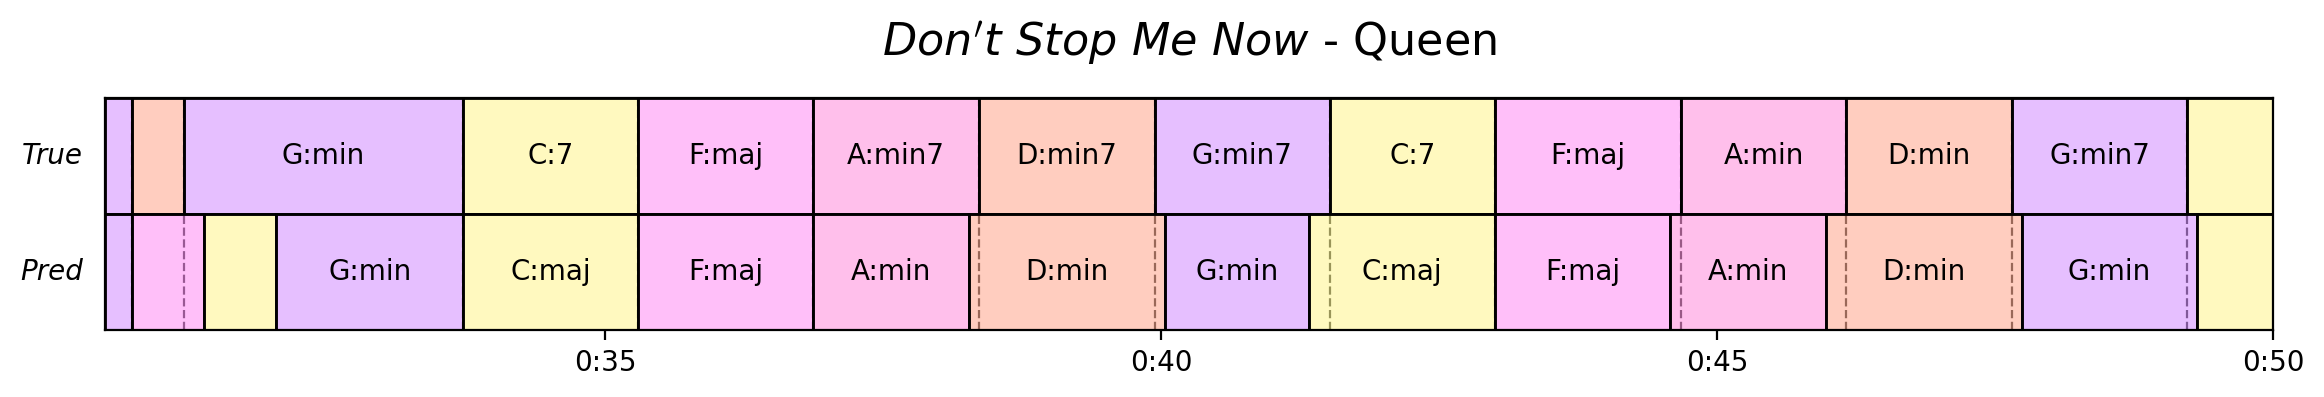
\includegraphics[width=1.0\textwidth]{figures/dontstopmenow.png}
    \caption{Comparison of predictions with ground truth on a section of \emph{Don't Stop Me Now} by Queen. Predictions have the correct root and third and are well timed but have discrepancies in sevenths. }\label{fig:dontstopmenow}
\end{figure}

The second song is \emph{Roxanne} by The Police, illustrated in Figure~\ref{fig:roxanne}. Syncopation, ambiguous bass, and sliding vocals make this song harder to annotate. Root recall is almost $80\%$ but \texttt{mirex} is only $64\%$. Sevenths are often omitted and thirds are sometimes wrong as well. The model confuses major and minor, and sus4 and major qualities. There are also some chord transitions which are not present in the ground truth and chord transitions are not all well-timed.

Overall, outputs are a lot smoother than found previously in Section~\ref{sec:crnn_examples} with more cohesive predictions of the same chord for a series of frames. However, the problem associated with identifying rarer chord qualities remains. Performance is also still highly song dependent. The model's accuracies over songs in the test set have a standard deviation of $20\%$. 

\begin{figure}[H]
    \centering
    % \hspace{-1.5cm}
    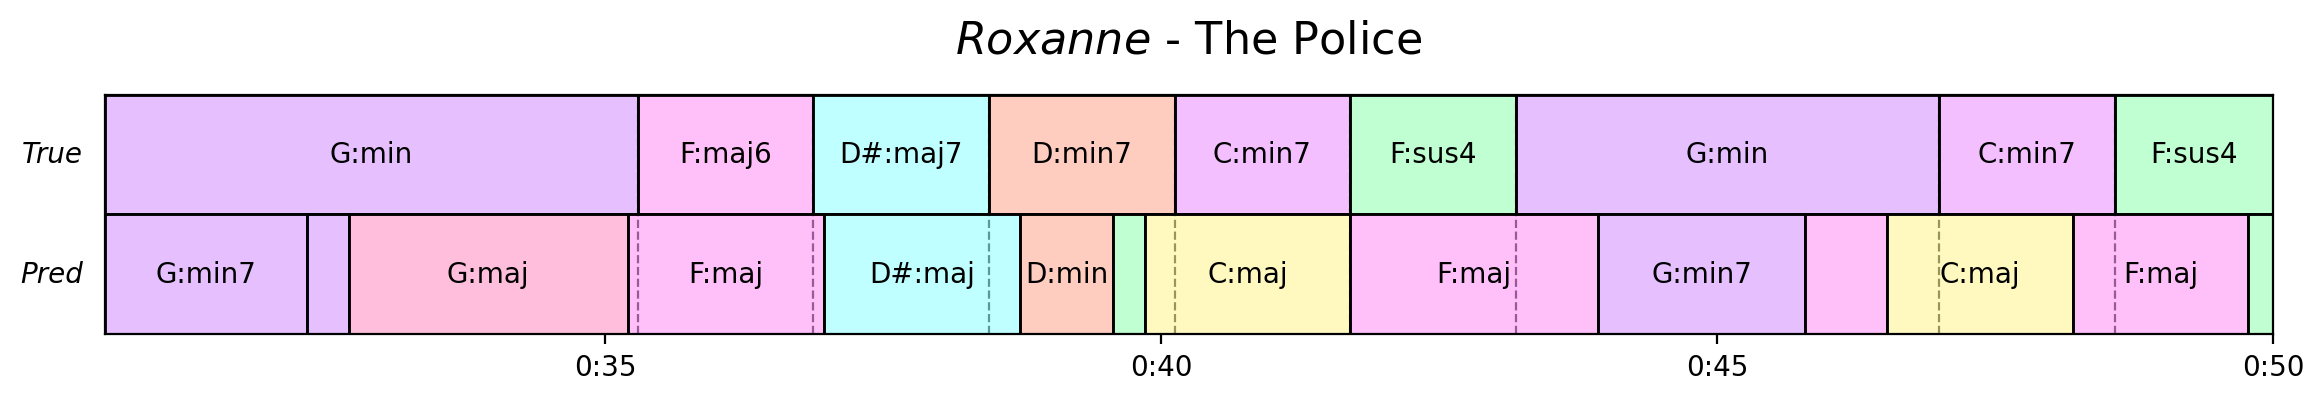
\includegraphics[width=1.0\textwidth]{figures/roxanne_thepolice.png}
    \caption{Comparison of predictions with ground truth on a section of \emph{Roxanne} by The Police. Predictions have the correct root but are not always well timed and do not always have the correct quality. The model's annotation is not very good on this song. }\label{fig:roxanne}
\end{figure}

As a final example, frame-wise and beat-wise predictions are compared on two songs not part of the dataset in Figure~\ref{fig:frame_vs_beat_wise}: \emph{Someone Like You} by Adele and \emph{Misty} by Ella Fitzgerald. In both cases, similar chord information is visualised differently. From a musicians' perspective, frame-wise predictions lead to ambiguity over how long a chord lasts in beats. Frame‑wise block lengths hint at beats but are not uniform. With time changes, this would become more problematic. In regions with rapid chord transitions, chords are not musically interpretable. In contrast, beat-wise predictions resemble musical notation more closely, and longer beat intervals prevent rapid chord changes. However, when predictions occur part-way through bars, beat-wise output can still be hard to interpret.

\begin{figure}[H]
    \centering
    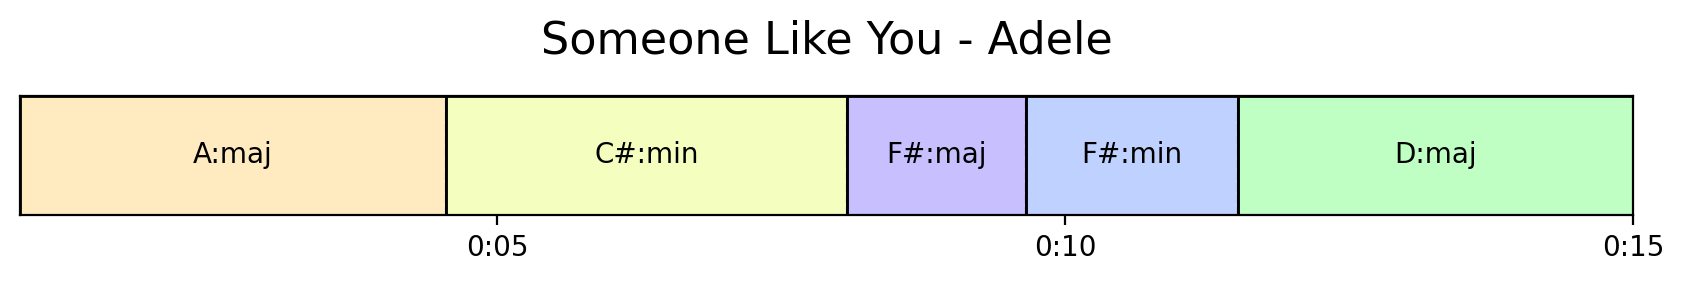
\includegraphics[width=1.0\textwidth]{figures/someone_like_you_chord.png}
    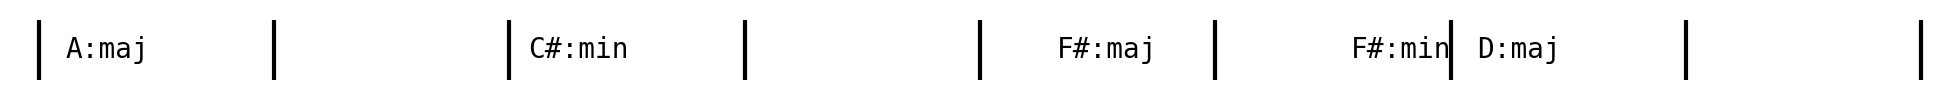
\includegraphics[width=1.0\textwidth]{figures/someone_like_you_chord_chart.png}\\
    \vspace{0.2cm}
    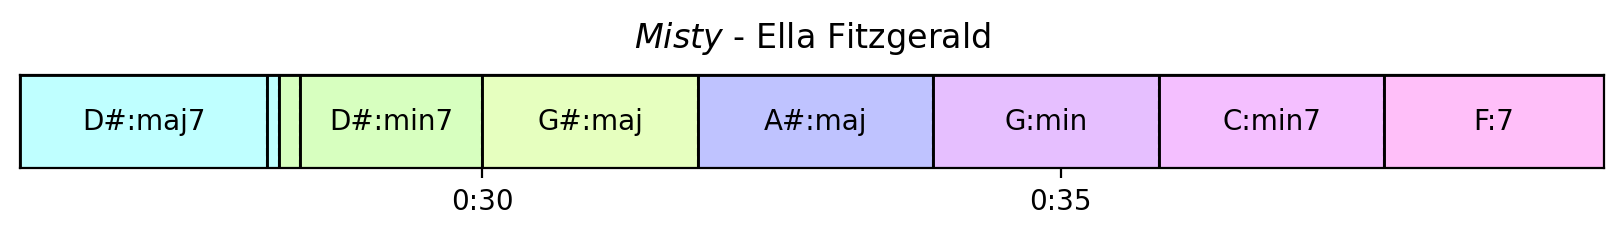
\includegraphics[width=1.0\textwidth]{figures/misty_chord_plot.png}
    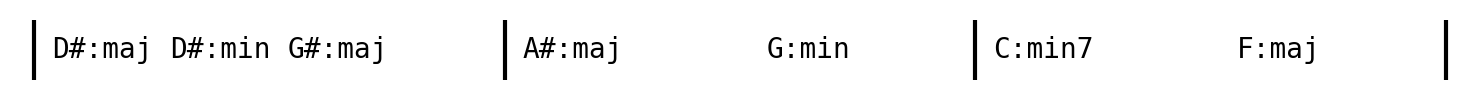
\includegraphics[width=1.0\textwidth]{figures/misty_chord_chart.png}
    \caption{Comparison of frame-wise and beat-wise predictions on \emph{Someone Like You} by Adele and \emph{Misty} by Ella Fitzgerald. Beat-wise predictions are visualised over bars with a meter of 4. For both methods, adjacent predictions of the same chord are grouped together. While beat-wise predictions are more musically meaningful and easily parsed, they can be messy and hard to interpret when chord transitions are late or off the beat.}\label{fig:frame_vs_beat_wise}
\end{figure}